\documentclass{article}

\usepackage[polish]{babel}
\usepackage{polski}
\usepackage[utf8]{inputenc}

\usepackage{indentfirst}

\usepackage{longtable}

\usepackage{float}

\usepackage[a4paper,top=2cm,bottom=2cm,left=3cm,right=3cm,marginparwidth=1.75cm]{geometry}

\usepackage{listings}

\usepackage{amsmath}
\usepackage{graphicx}
% \usepackage[colorlinks=true, allcolors=blue]{hyperref}

\title{Raport z Ćwiczenia 2}
\author{Bartłomiej Rasztabiga 304117}

\begin{document}
\maketitle

\section{Treść zadania}

Zaimplementuj strategię ewolucyjną typu \begin{math}(\mu/\mu, \lambda)\end{math}-ES, w której rozważysz dwa mechanizmy adaptacji zasięgu mutacji:
\begin{itemize}
  \item samoadaptację (ang. Self-Adaptation, SA)
  \item metodę logarytmiczno-gaussowską (ang. Log-Normal Mutation Rule, LMR).
\end{itemize}

Następnie zbadaj zbieżność obu metod w zależności od rozmiaru populacji potomnej oraz początkowej wartości zasięgu mutacji.

\section{Opis implementowanego algorytmu}

Poniżej przedstawiam pseudokod wykorzystanej strategii ewolucyjnej.
Zastosowanym warunkiem zakończenia ewolucji jest osiągnięcie maksymalnej liczby iteracji.

\begin{lstlisting}[language=Python,mathescape=true]
iteration = 0
avg_point = Individual(initial_point, initial_sigma)

while iteration < max_iteration:
    generate_lambda_individuals()  # generowanie $\lambda$ kopii avg_point
    sigma_adaptation()             # adaptacja $\sigma$: LMR lub SA
    mutation()                     # mutacja: x + $\sigma$ * $\mathcal{N}_{i}(0, \pmb{I}_{D})$
    grade_population()             # ocena populacji
    succession()                   # sukcesja - $\mu$ najlepszych osobnikow
    recombination()                # wyliczenie avg_point

    update_best_so_far()           # aktualizacja najlepszego osobnika

return best_so_far, iteration
\end{lstlisting}

\section{Opis planowanych eksperymentów numerycznych}

\subsection{Porównanie najlepszych osobników z algorytmów LMR i SA}

Pierwszym planowanym eksperymentem będzie porównanie wyjściowego najlepszego osobnika dla obu algorytmów adaptacji: samoadaptacji i LMR. Zastosowano różne wartości $\mu$ i $\sigma$.
$\mu \in \{2, 10, 100\}$,  $\sigma \in \{0.1, 1, 10\}$

Do celów porównania jakości obu algorytmów adaptacji sigmy wykorzystałem poniższe dwie funkcje:

\begin{itemize}
  \item f(x) - funkcja sferyczna wyrażona wzorem $f(\textbf{x}) = \sum^{n}_{i = 1}x^{2}_{i},\; \textbf{x}\in [-100, 100]^{D}$
  \item g(x) - funkcja "happy cat" wyrażona wzorem $q(\pmb{x}) = [(\|\pmb{x}\|^{2} - D)^{2}]^{1/8} + D^{-1}(\frac{1}{2}\|x\|^{2} + \sum^{D}_{i = 1}x_{i}) + \frac{1}{2},\; \pmb{x} \in [-100, 100]^{D}$
\end{itemize}

W obu przypadkach parametr D (wymiarowość) równy jest 10.

\subsection{Porównanie zbieżności algorytmów LMR i SA}

Drugim planowanym eksperymentem będzie porównanie ocen uśrednionych osobników w czasie dla obu algorytmów adaptacji. Zastosowano takie same wartości $\mu$ i $\sigma$ oraz funkcje kosztu jak w eksperymencie numer 1.

\section{Opis uzyskanych wyników}

\subsection{Porównanie najlepszych osobników z algorytmów LMR i SA}

W kolumnach LMR i SA podane są finalne oceny uśrednionych osobników, odpowiednio dla algorytmu LMR i samoadaptacji. Porównanie dokonane jest dla obu funkcji: f(x) i q(x).

\begin{center}
\begin{longtable}{|c c c c|}
\caption{f(x) - funkcja sferyczna} \\
\hline
mi & sigma & LMR & SA \\
\hline \hline
2 & 0.1 & 9.241e+03 & 1.285e-03 \\
\hline2 & 1 & 1.610e+03 & 1.180e-11 \\
\hline2 & 10 & 4.989e+01 & 9.722e-13 \\
\hline\hline10 & 0.1 & 1.083e+04 & 3.717e-25 \\
\hline10 & 1 & 3.196e+01 & 1.626e-38 \\
\hline10 & 10 & 2.068e-01 & 1.426e-41 \\
\hline\hline100 & 0.1 & 2.242e+03 & 1.306e-38 \\
\hline100 & 1 & 2.046e-04 & 3.339e-48 \\
\hline100 & 10 & 6.267e-04 & 1.207e-51 \\
\hline

\end{longtable}
\end{center}

\begin{center}
\begin{longtable}{|c c c c|}
\caption{q(x) - funkcja happy cat} \\
\hline
mi & sigma & LMR & SA \\
\hline \hline
2 & 0.1 & 2.075e+02 & 1.579e+00 \\
\hline2 & 1 & 7.426e+01 & 1.541e+00 \\
\hline2 & 10 & 4.746e+00 & 1.596e+00 \\
\hline\hline10 & 0.1 & 4.535e+02 & 1.003e+00 \\
\hline10 & 1 & 2.048e+01 & 1.046e+00 \\
\hline10 & 10 & 7.903e-01 & 1.032e+00 \\
\hline\hline100 & 0.1 & 4.191e+02 & 5.574e-01 \\
\hline100 & 1 & 6.744e-01 & 5.780e-01 \\
\hline100 & 10 & 9.391e-01 & 5.592e-01 \\
\hline

\end{longtable}
\end{center}

\begin{figure}[H]
\caption{Wartość funkcji f(x) dla uśrednionego osobnika wynikowego ES, początkowa $\sigma$=0.1}
\centering
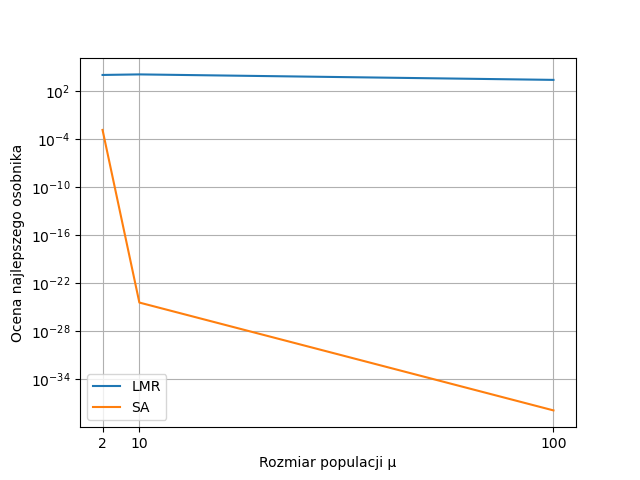
\includegraphics[scale=0.8]{func=f sigma=0.1.png}
\end{figure}

\begin{figure}[H]
\caption{Wartość funkcji f(x) dla uśrednionego osobnika wynikowego ES, początkowa $\sigma$=1}
\centering
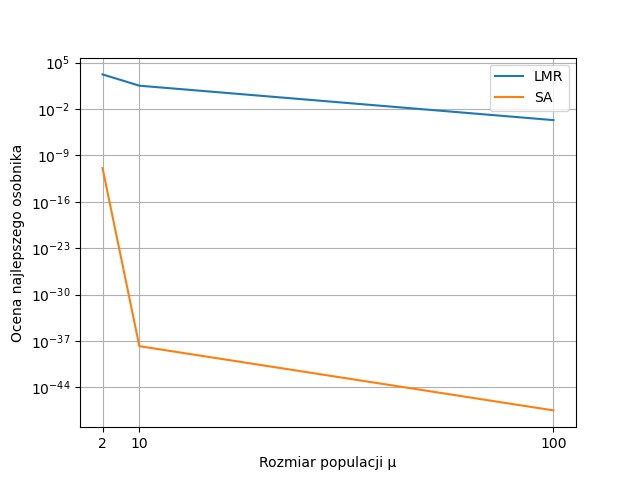
\includegraphics[scale=0.8]{func=f sigma=1.png}
\end{figure}

\begin{figure}[H]
\caption{Wartość funkcji f(x) dla uśrednionego osobnika wynikowego ES, początkowa $\sigma$=10}
\centering
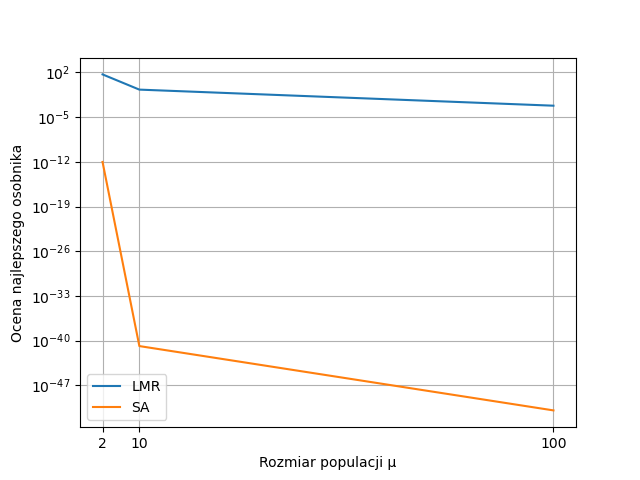
\includegraphics[scale=0.8]{func=f sigma=10.png}
\end{figure}

\begin{figure}[H]
\caption{Wartość funkcji q(x) dla uśrednionego osobnika wynikowego ES, początkowa $\sigma$=0.1}
\centering
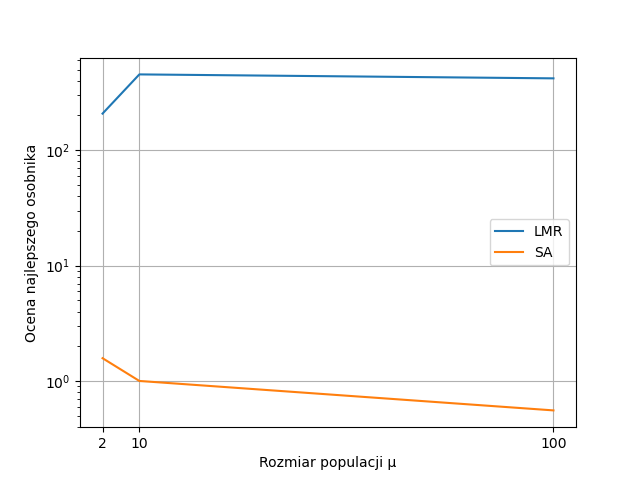
\includegraphics[scale=0.8]{func=q sigma=0.1.png}
\end{figure}

\begin{figure}[H]
\caption{Wartość funkcji q(x) dla uśrednionego osobnika wynikowego ES, początkowa $\sigma$=1}
\centering
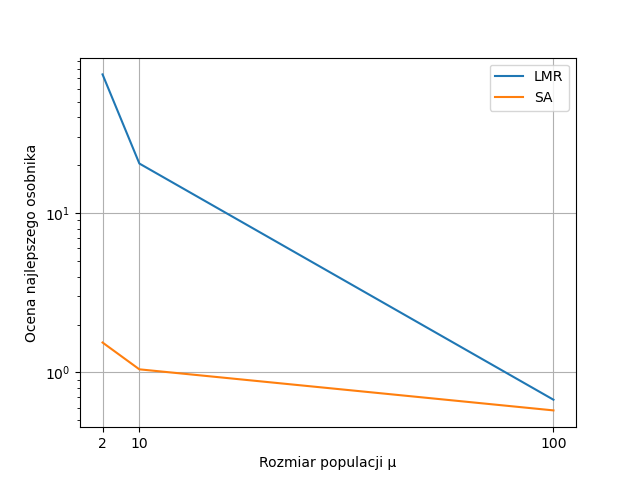
\includegraphics[scale=0.8]{func=q sigma=1.png}
\end{figure}

\begin{figure}[H]
\caption{Wartość funkcji q(x) dla uśrednionego osobnika wynikowego ES, początkowa $\sigma$=10}
\centering
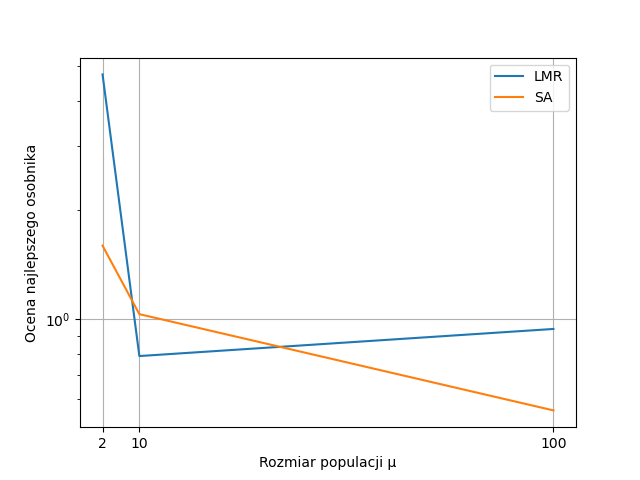
\includegraphics[scale=0.8]{func=q sigma=10.png}
\end{figure}

\subsection{Porównanie zbieżności algorytmów LMR i SA}

Wyniki drugiego eksperymentu przedstawione są w postaci zgrupowanych wykresów przedstawiających wartości funkcji kosztu dla każdej iteracji, przez co można zaobserwować zbieżność lub rozbieżność metody. W kolumnach przedstawione są wykresy dla takich samych wartośći $\mu$ a w wierszach dla $\sigma$. Na osi x podane są iteracje (w tym przypadku są to wartośći od 0 do 1000), a na osi y przedstawiono wartość funkcji kosztu dla uśrednionego osobnika populacji wynikowej.

\begin{figure}[H]
\caption{Wartość funkcji f(x) dla uśrednionego osobnika w czasie}
\centering
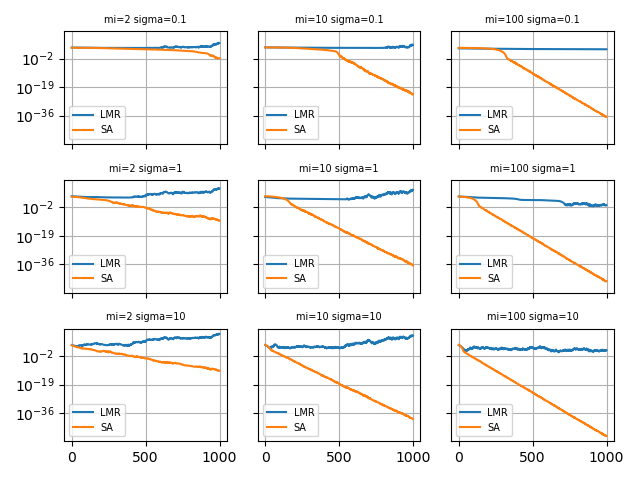
\includegraphics[scale=0.8]{conv func=f.png}
\end{figure}

\begin{figure}[H]
\caption{Wartość funkcji q(x) dla uśrednionego osobnika w czasie}
\centering
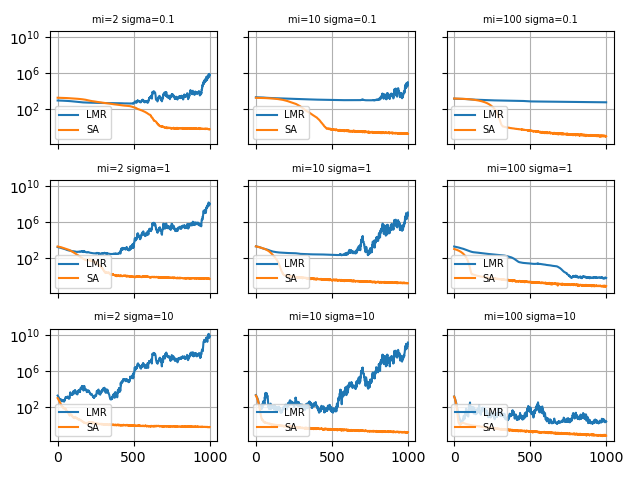
\includegraphics[scale=0.8]{conv func=q.png}
\end{figure}

\section{Wnioski z przeprowadzonych badań}

\subsection{Porównanie najlepszych osobników z algorytmów LMR i SA}

Algorytm samoadaptacji oferuje znacząco lepsze wyniki niż algorytm LMR. Jest to spowodowane różnicą w implementacji, polegającą na uśrednianiu sigmy podczas uśredniania populacji (w trakcie rekombinacji). Z tego powodu kolejna sigma wyliczana jest na podstawie sigmy, służącej do wyliczenia lepszej części populacji (po sukcesji elitarnej).

Ponadto można zauważyć, że wyższe wartości początkowej $\sigma$ z reguły powodują szybsze zbieganie algorytmu. Jednakże w przypadku zastosowania za wysokiej $\sigma$, algorytm LMR powoduje znaczące rozbieganie kolejnych populacji. Algorytm samoadaptacji, jak nazwa wskazuje, posiada zdolności zmniejszania zbyt wysokiej $\sigma$, przez co nie ma to tak negatywnego efektu jak w przypadku LMR.

W przypadku różnych wartości $\mu$ można zaobserwować poprawę jakości działania algorytmu wraz ze wzrostem rozmiaru populacji, chociaż wiąże się to z wydłużeniem czasu działania.

\subsection{Porównanie zbieżności algorytmów LMR i SA}

Z wykresów zbieżności algorytmów LMR i SA można zauważyć, że algorytm samoadaptacji zachowuje się bardzo dobrze w sytuacji wysokiej $\mu$ i $\sigma$. Nie występują w nim również oscylacje ani odbieganie od minimum funkcji kosztu.

Algorytm LMR w większości przypadków od pewnej iteracji "ucieka" w zbyt wysokie wartości funkcji lub zatrzymuje się w pewnym punkcie.

W przypadku funkcji f(x) algorytm LMR jest w stanie znaleźć punkt bliski minimum globalnemu, jednakże SA uzyskuje w tych przypadkach znacząco wyższą dokładność.

\end{document}